\chapter{Dimensionality Reduction}
L'obiettivo, è quello di trattare un dataset D-dimensionale, come uno K-dimensionale, con $K << D$.

\section{Multi Dimensional Scaling (DMS)}
Assegnare gli elementi in uno spazio K-dimensionale, cercando di minimizzare lo stress.

\begin{defn}[Stress]
  Qaundo il nuovo punto mantiene le informazioni del vecchio:
  \[
    \text{stress} = \sqrt{\frac{\sum_{i,j} (\hat{d}_{ij} - d_{ij})^2}{\sum_{i,j} d_{ij}^2}}, \; d_{ij} = |o_j - o_i|
  \]
  Dove $d$ rappresenta la distanza tra $i$ e $j$.
\end{defn}
Si vuole minimizzare lo stress per ogni punto, ma ha una complessità computazionale di:
\begin{itemize}
  \item \textbf{$O(N^2)$} a running time.
  \item \textbf{$O(N)$} per aggiungere un oggetto.
\end{itemize}

Ci sono due riduzioni principali:
\begin{itemize}
  \item \textbf{Isometrico}, mantiene la distanza:
    \[
      D'(F(i), F(j)) = D(i,j)
    \]
  \item \textbf{Contrattivo}, diminuisce la distanza:
    \[
      D'(F(i), F(j)) \le D(i,j)
    \]
\end{itemize}

\subsection{PCA}
Una tecnica di riduzione lineare, divisa in diverse fasi:
\begin{enumerate}
  \item Creazione di una matrice $X = N \times d$.
  \item Sottarre a ogni $x_n$ il valore $x_medio$ della matrice $X$.
  \item Calcolare la covarianza $\Sigma$ della matrice $X$. Dato $\Sigma = AA^T \; \text{dove} \; A = [r_1, \cdots, r_m]$.
  \item Calcolare gli autovettori e gli autovalori della covarianza $\Sigma$. Dato:
    \begin{enumerate}
      \item \textbf{Autovalore:} $Av = \lambda v$.
      \item \textbf{Autovettore:} $AA^T(Av_i) = \mu_i(Av_i)$ oppure $A^TAv_i = \mu_iv_i$.
    \end{enumerate}
  \item Scegliere gli $M$ autovettori più grandi, nello specifico ogni coppia di autovettori deve avere covarianza zero.
  \item Proiettare i dati in uno spazio K-dimensionale: $p = U^T(x - \mu)$.
\end{enumerate}

\begin{note}[Nota Bene]
  Se ci sono grandi quantita di dati, come per esempio un numero di immagini maggiore di $10^4$, si può notare che la covarianza ha una dimensione di $d^2$,
  quindi si avrebbe $d \ge 10^4$ con $\Sigma \ge 10^8$.
\end{note}

\subsection{Riduzione non Lineare}

\begin{defn}[Manifold]
  Un manifold è uno spazio topologico localmente euclideo. In generale, qualsiasi oggetto che sia quasi piatto su piccola scala.
\end{defn}

\begin{defn}[Embedding]
  Un embedding è una rappresentazione di un oggetto topologico,
  di una varietà, di un grafo, di un campo, in un determinato spazio,
  tale da preservarne la connettività o le proprietà algebriche. \\
  Per esempio, gli insiemi dei numeri reali, razionali e interi.
\end{defn}

\begin{defn}[Geodesic]
  La curva più breve su un manifold che congiunge due punti del manifold stesso. \\
  Ha una sua lunghezza ed è utile perchè la distanza euclidea tende a non essere molto buona.
\end{defn}

\begin{figure}[!htb]
    \centering
    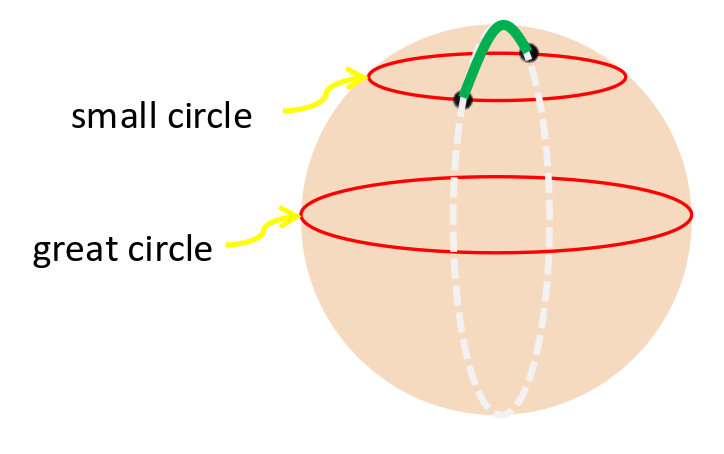
\includegraphics[width=0.4\linewidth]{Images/dim_reduction/geodesic.png}
    \caption{Rappresentazione di un geodesic in una sfera.}
\end{figure}

\subsection{LLE e Laplacian Eignmap}
Algoritmo basato su grafi e ha tre fasi:
\begin{enumerate}
  \item Trovare $K$ vicini per ottenere un manifold, rapprensentato con una laplaciana e tramite un grafico dei punti vicini.
  \item Stimare le proprietà del manifold guardando i punti vicini.
  \item Cercare un embedding globale che mantiene le proprietà trovate.
\end{enumerate}
Per costruire la lagrangiana, abbiamo bisogno di una matrice $W$, quella dei pesi, che definisce quando è importante il collegamento tra due nodi.
Ci sono due modi per calcolare la matrice dei pesi:
\begin{enumerate}
  \item \textbf{Metodo semplice:} 0 se non c'è collegamento, 1 se è presente.
  \item \textbf{Head Kernel:} considera l’importanza dei collegamenti presenti $A_{ij} = e^{-\frac{\|x_i - x_j\|^2}{t}}$.
\end{enumerate}
Possiamo trovare il manifold ottimale, ottimizzando:
\[
  \arg\min_Y \text{trace}(Y'LY)
\]
La soluzione sono i primi $m$ autovettori.
